%%%%%%%%%%%%%%%%%%%%%%%%%%%%%%%%%
\subsection{Introduction}
\label{sec:fdsp-slow-cryo-intro}

% RC:
% - Clarity could be increased by making the document more consistent about what systems are included in the CISC scope. Figure 1.1 contains several items that are not mentioned elsewhere in the document: "Instrumentation Feed-throughs," "Feedthrough contamination studies," and "Instrumentation Precision Studies."
% - Firmware and racks are mentioned in the introduction but not elaborated on much later in the document or included in Fig. 1.1.
% - E-field simulations are mentioned in the Introduction and Interface sections but not described in the main body (Sec. 1.2 and 1.3).
% - A clear statement in words (or as a boundary on Fig. 1.1) of the exact border between DUNE and LBNF would be very helpful. One particularly unclear point is whether feed-throughs are the responsibility of DUNE or LBNF.


% identical for SP and DP 
The Cryogenic Instrumentation and Slow Controls (CISC) system provides
a comprehensive monitoring for all detector components as well as for the liquid argon quality and behavior, both being crucial
to guaranty a good quality of the data. CISC also provides a control system for some of the detector components. 
The structure of the CISC consortium is quite complex. A subsystem chart
for the CISC system is shown in Fig. \ref{fig:sp-slow-cryo-subsys}. 

\begin{dunefigure}[Cryogenic Instrumentation and Slow Controls (CISC) subsystems]{fig:sp-slow-cryo-subsys}
{Cryogenic Instrumentation and Slow Controls (CISC) subsystem chart}
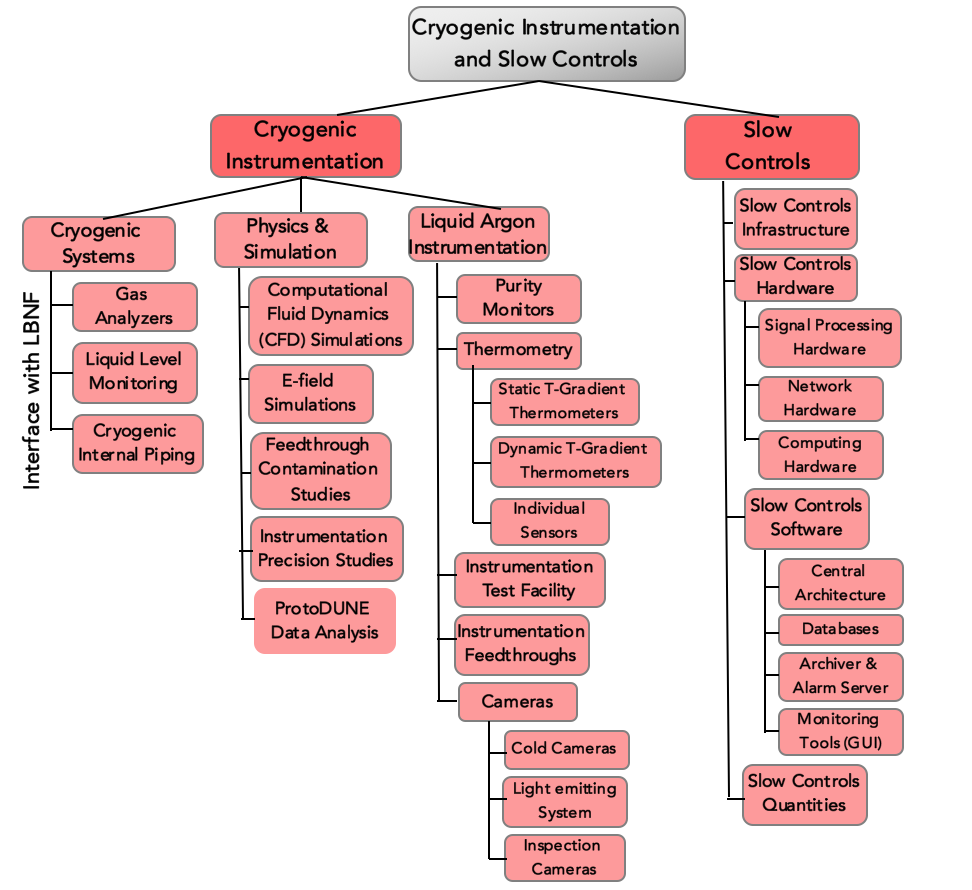
\includegraphics[width=0.7\textwidth]{cisc_subsys}
\end{dunefigure}

Two main branches can be distinguished: i) Cryogenics Instrumentation and ii) Slow Controls. The former includes a set of devices 
to monitor the quality/behavior of the liquid argon volume in the cryostat interior, ensuring the correct functioning of
the cryogenics system and the suitability of the LAr for good quality physics data. Those devices are:
purity monitors, temperature monitors, gas analyzers, liquid argon level monitors, cameras and their associated
light emitting system. Two other systems have been included as part of the Cryogenics Instrumentation,  
a test facility for the instrumentation devices and the cryogenic piping inside the cryostat.

Cryogenic Instrumentation also requires significant physics and
simulation work such as E-field simulations and cryogenics modeling
studies using Computational Fluid Dynamics (CFD). E-field simulations
are required to identify desirable locations for instrumentation
devices in the cryostat such that they are not in regions of high electric potential and
that the designs do not induce large field distortions. CFD
simulations are needed to understand the expected temperature,
impurity and velocity flow distributions and guide the placement and
distribution of instrumentation devices inside the cryostat.


From the organizational point of view
Cryogenics Instrumentation has been devided in three main parts: i) Cryogenics Systems, which includes all components directly related with the external cryogenic system as
liquid level monitoring, gas analysers and internal cryogenics piping, all having substancial interfaces with LBNF, ii) Liquid Argon Instrumentation, which includes all
other subsystemsinstrumentation devices, and iii) Physics and Simulation, ...


The second branch of CISC is the Slow Controls system, in charge of monitoring and control most detector elements, as power supplies, electronics, racks, instrumentation devices,
calibration devices, etc. It includes four main components: hardware, infrastructure,
software and firmware. The slow controls hardware and infrastructure consists of
networking hardware, signal processing hardware, computing hardware and relevant
rack infrastructure. The slow controls software and firmware will be needed for
signal processing, alarms, archiving and control room displays.

%The instrumentation work related to gas analyzers, liquid level
%monitors and internal cryogenic piping has significant
%interface with LBNF and will be coordinated between DUNE and LBNF.


%%%%%%%%%%%%%%%%%%%%%%%%%%%%%%%%%%%%%
\subsection{Design Considerations}
\label{sec:fdsp-slow-cryo-des-consid}

% specific to SP

For all liquid argon instrumentation devices, ProtoDUNE designs are
considered as baseline and requirements for most design
parameters are extrapolated from ProtoDUNE. Hence a critical step for
the CISC consortium is to analyze data from ProtoDUNE when available
to validate the instrumentation designs and understand their
performance. Some of the common design considerations for
instrumentation devices include stability, reliability and longevity
such that the devices can survive for a period of at least 20 years
(current official DUNE run time).  Since it is uncommon for any device
to have such a long lifetime, provisions will be made in the overall
design to allow replacement of devices after certain number of
years whenever is possible. The noise from instrumentation devices need to be kept at the
ALARA level where ALARA stands for As Low As Reasonably
Achievable. The electric field on the instrumentation devices is 
required to be less than \SI{30}{kV\per\cm},
such that the risk of dielectric breakdown in LAr is minimized, what implies 
the ussage of E-field shielding for devices in regions of high electric potential. 
Another common consideration for all instrumentation devices is their support structure
design which is expected to be substantially different from the one used in ProtoDUNE.

For slow controls, the system needs to be designed such that it is
robust enough to support large number of variables, broad range of
monitoring and archiving rates and has the capability to interface
with large number of systems to establish two-way communication for
control and monitoring. Table \ref{tab:sp-cisc-requirements} shows
some of the important CISC system design requirements.
%A full list of requirements for design parameters can be found in
%DUNE Doc-DB 6440.


\begin{dunetable}
[Important design requirements on the SP CISC system design]
{p{0.22\textwidth}p{0.17\textwidth}p{0.32\textwidth}p{0.19\textwidth}}
{tab:sp-cisc-requirements}
{Important design requirements on the single phase CISC system design}
Design Parameter
 & Requirement
 & Motivation
 & Requirement met?
\\ \toprowrule
Electron lifetime measurement precision
 & $<\SI{1.4}{\%}$
 & Per DUNE-FD Task Force, needed to keep the bias on the charge readout in the TPC to below \SI{0.5}{\%} at \SI{3}{ms}
 & Yes: existing purity monitors; extrapolation to TPC under development
\\  \colhline
Thermometers precision
 & $<\SI{5}{mK}$
& Driven by CFD simulation validation; based on ProtoDUNE-SP design
& Yes: ProtoDUNE thermometers \SI{2}{mK}
\\ \colhline
Thermometers density
 & \(>2/\si{m}\) (vert.), \(\sim\)~0.2/\si{m} (horiz.)
 & Driven by CFD simulation
 & Yes: design
\\ \colhline
Liquid level meters precision (SP)
 & \SI{0.1}{\%} over \SI{14}{m}
& Standard sensitivity; two level meters for redundancy
& Yes: design calculation
\\  \colhline
% Liquid level meters precision (DP)
%  & \(<\SI{1}{mm}\)
% & Maintain constant gas phase drift
% & Yes: WA105 / ProtoDUNE-DP design \SI{0.1}{mm}
% \\  \colhline
 Cameras
 & \multicolumn{3}{p{0.64\textwidth}}{see Table \ref{tab:fdgen-cameras-req}}
 \\ \colhline
Cryogenic Instrumentation Test Facility cryostat volumes
 & 0.5 to \SI{3}{m^3}
& Based on filling costs and turn around times
& Under design
\\  \colhline
 Max.\ E-field on instrumentation devices
 & \(<\SI{30}{kV/cm}\)
 & The mechanical design of the system should be such that E-field is below this value, 
 to minimize the risk of dielectric breakdown in LAr
 & Yes: electrostatic simulation
\\ \colhline
 Minimize noise from instrumentation devices
 & ALARA
 & Keep readout electronics free from external noise, which confuses event reconstruction (As Low As Reasonably Achievable)
\\ \colhline
Alarm rate
 & \(<\SI{150}{\per\day}\)
& Recommended manageable alarm rate; allows experiment operators to respond to every alarm.
& To be met by design of connected systems
\\  \colhline
Total no.\ of variables
 & 50k to 100k
& Expected number based on scaling past experiments; requires robust base software model that can handle large no. of variables.
& Yes: existing control system software; DUNE choice in progress.
\\  \colhline
Max.\ archiving rate per channel
 & \SI{1}{Hz} (burst), \SI{1}{\per\minute} (avg.)
& Based on expected rapidity of interesting changes; impacts the base software choice; depends on data storage capabilities
& Yes: existing control system software; DUNE choice in progress.
\\ \colhline
Near Detector  status
 & Full Beam and Detector Status
& Operate DUNE as one experiment.
& Yes: IFBeamDB, internet
\\
% 
% 
% 
% Requirement  
%   \\ \colhline
%    \\ \colhline
%  ...\\ 
\end{dunetable}

% \fixme{By the end of the volume, for every requirement listed in this section, there should exist an explanation of how it will be satisfied.}


%%%%%%%%%%%%%%%%%%%%%%%%%%%%%%%%
\subsection{Scope}
\label{sec:fdsp-slow-cryo-scope}

% identical for SP and DP

The scope of the CISC system spans over a broad range of activities. In the
case of Cryogenics Systems (gas analyzers, liquid level monitors and
cryogenic internal piping), LBNF will provide the needed expertise and
is responsible for the design, installation and commissioning activities
while the CISC consortium provides the cost and supplement the labor as
needed. In the case of LAr Instrumentation Devices (purity monitors,
thermometers, cameras, and light emitting system) and instrumentation
test facility, CISC will be responsible from design to commissioning in
the far detectors.

From the slow controls side, CISC will provide control and monitoring of
all detector elements that provide information on the health of the
detector or conditions important to the experiment.
The scope of systems that slow controls includes is listed below:

\begin{itemize}
\item {\bf Slow Controls Base Software and Databases}: provides the central tools needed to develop control and monitoring for various detector systems and interfaces
  \begin{itemize}
  \item Base Input/Output software
  \item Alarms; archiving; display panels; operator interface tools
  \item Slow controls system documentation and operations guidelines
  \end{itemize}
\item {\bf Slow Controls for External Systems}: export data from systems external to the detector and provide status to operators and archiving
  \begin{itemize}
  \item Beam Status; Cryogenics status; DAQ status; Facilities systems
  \item building controls; Detector hall monitoring; ground impedance monitoring
  \item Interlock status bit monitoring (not the actual interlock mechanism)
  \end{itemize}
\item {\bf Slow Controls for Detector Hardware Systems}: develop software interfaces for detector hardware devices
  \begin{itemize}
  \item Monitoring and control of all power supplies
  \item Full rack monitoring (rack fans, thermometers and rack protection system)
  \item Instrumentation and Calibration device monitoring (and control to the extent needed)
  \item Power distribution units monitoring; Computer hardware monitoring
  \item High voltage system monitoring through cold cameras
  \item Detector components inspection through warm cameras
  \end{itemize}
\end{itemize}

In terms of slow controls hardware, CISC will develop, install and
commission any hardware related to rack monitoring and control. While
most power supplies might only need a cable from the device to an
ethernet switch, some power supplies might need special cables (e.g.
GPIB or RS232) for communication. The CISC consortium is responsible for
buying such control cables.

In addition to the listed activities, CISC also has activities that span
outside the scope of the consortium and require interfacing with other
groups. This is discussed in Sec. \ref{sec:fdgen-slow-cryo-intfc}.

% More specific information on how CISC scope of activities
% interface with other consortia can be found at DUNE Doc-dbs 6679 (APA),
% 6730 (SP-PD), 6745 (SP-CE), 6760 (DP-CRP), 6781 (DP-PD), 6784 (DP-CE),
% 6787 (HV), and 6790 (DAQ). The CISC interface documents with facility,
% installation, integration, calibration, and physics can be found at DUNE
% Doc-dbs 6991, 7018, 7045, 7072, and 7099, respectively. The CISC
% interface document with software and computing can be found at DUNE
% Doc-db 7126.
